% !TEX TS-program = pdflatex
% !TEX encoding = UTF-8 Unicode

% This is a simple template for a LaTeX document using the "article" class.
% See "book", "report", "letter" for other types of document.

\documentclass[10pt]{article} % use larger type; default would be 10pt

\usepackage[utf8]{inputenc} % set input encoding (not needed with XeLaTeX)

%%% Examples of Article customizations
% These packages are optional, depending whether you want the features they provide.
% See the LaTeX Companion or other references for full information.

%%% PAGE DIMENSIONS
\usepackage{geometry} % to change the page dimensions
\geometry{letterpaper} % or letterpaper (US) or a5paper or....
% \geometry{margin=2in} % for example, change the margins to 2 inches all round
% \geometry{landscape} % set up the page for landscape
%   read geometry.pdf for detailed page layout information

\usepackage{graphicx} % support the \includegraphics command and options

% \usepackage[parfill]{parskip} % Activate to begin paragraphs with an empty line rather than an indent

%%% PACKAGES
\usepackage{booktabs} % for much better looking tables
\usepackage{array} % for better arrays (eg matrices) in maths
\usepackage{paralist} % very flexible & customisable lists (eg. enumerate/itemize, etc.)
\usepackage{verbatim} % adds environment for commenting out blocks of text & for better verbatim
\usepackage{subfig} % make it possible to include more than one captioned figure/table in a single float
% These packages are all incorporated in the memoir class to one degree or another...

%%% HEADERS & FOOTERS
\usepackage{fancyhdr} % This should be set AFTER setting up the page geometry
\pagestyle{fancy} % options: empty , plain , fancy
\renewcommand{\headrulewidth}{0pt} % customise the layout...
\lhead{}\chead{}\rhead{}
\lfoot{}\cfoot{\thepage}\rfoot{}

%%% SECTION TITLE APPEARANCE
\usepackage{sectsty}
\allsectionsfont{\sffamily\mdseries\upshape} % (See the fntguide.pdf for font help)
% (This matches ConTeXt defaults)

%%% ToC (table of contents) APPEARANCE
\usepackage[nottoc,notlof,notlot]{tocbibind} % Put the bibliography in the ToC
\usepackage[titles,subfigure]{tocloft} % Alter the style of the Table of Contents
\renewcommand{\cftsecfont}{\rmfamily\mdseries\upshape}
\renewcommand{\cftsecpagefont}{\rmfamily\mdseries\upshape} % No bold!

\usepackage{siunitx} % Required for alignment

\sisetup{
  %round-mode         = places, % Rounds numbers
  %round-precision     = 5, % to 6 places
table-format=1.5
}

\usepackage[round,authoryear,sort,comma]{natbib}


%%% END Article customizations

%%% The "real" document content comes below...

\title{A Closer Look at the Size of the Coronavirus Disease 2019}
\author{Andrea Capra}
%\date{} % Activate to display a given date or no date (if empty),
         % otherwise the current date is printed 

\begin{document}
\maketitle

\section{Filtration Efficiency}
Three main mechanism are responsible forthe filtration of aerosol particles by fibrous filters. For submicron particles the dominant process is collection by Brownian diffusion. For larger particles interception and inertial impaction mechanisms are active. It results that there exists a region where none of the above effects predominates over the others, yielding a maximum in the particle penetration, and consequently a minimum in the filtration efficiency. Whilethe location of said minimum depends on the type of filter and the flow velocity, it generally occcurs around $0.3\,\mu$m. In addition it's worth noting that the most penetrating particle size will decrease with increasing filtration velocity and increase with increasing filter fiber size. Further, it predicts that increasing the filter solid volume fraction. For explicit calculation see \cite{lee1980} and references therein.

\section{Dust Mask and Filter Cartridge Ratings}

See Table~\ref{tab:respirator_rating} for a classification of filtering respirators by the U.S. National Institute for Occupational Safety and Health (NIOSH). 

\begin{table}[h!]
  \begin{center}
    \caption{NIOSH Particulate Respirator Class Minimum Efficiency Levels. The diameter referes to the \textit{mass-median-diameter}, identified by the symbol $D_{50}$, and is considered to be the average particle diameter by mass}
    \label{tab:respirator_rating}
    \begin{tabular}{p{0.1\textwidth}p{0.3\textwidth}|p{0.1\textwidth}p{0.4\textwidth}}
      \toprule % <-- Toprule here
      \multicolumn{4}{c}{\textbf{Respirator Rating}}\\
	\multicolumn{2}{c}{Letter Class}&\multicolumn{2}{c}{Number Class}\\
       \midrule % <-- Midrule here
	 N & Not oil resistant  & 95 & Removes 95\% of all particles that are at least $0.3\,\mu$m in diameter\\
           R & Resistant to oil    & 99 & Removes 99\% of particles that are at least $0.3\,\mu$m in diameter\\
           P & Oil Proof              & 100 & Removes 99.97\% of all particles that are $0.3\,\mu$m in diameter or larger\\
     \bottomrule % <-- Bottomrule here
    \end{tabular}
  \end{center}
\end{table}


\section{Example Particle Sizes}

See Table~\ref{tab:particle_sizes}.

\noindent
Source: https://www.envirosafetyproducts.com/resources/dust-masks-whats-the-difference.html


\begin{table}[h!]
  \begin{center}
    \caption{Example Particle Sizes}
    \label{tab:particle_sizes}
    \begin{tabular}{lSS}
      \toprule % <-- Toprule here
      \textbf{Particle} & \textbf{Min Diamteter} &  \textbf{Max Diamteter}\\
	& \multicolumn{2}{c}{$\mu$m}\\
      \midrule % <-- Midrule here
	Anthrax                                & 1 & 5\\
	Asbestos                              & 0.7 & 90\\
	Atmospheric Dust                   & 0.001 & 40\\
	Bacteria                                & 0.3 & 60\\
	Beach Sand                           & 100 & 10000\\
	Bone Dust                             & 3 & 300\\
	Bromine 	                              & 0.1 & 0.7\\
	Carbon Dioxide                       & \multicolumn{2}{S}{0.00065}\\
	Copier Toner 	                        & 0.5 & 15\\
	Corn Starch 	                        & 0.1 & 0.8\\
	Fiberglass Insulation                 & 1 & 1000\\
	Lead 	                              & 0.1 & 0.7\\
	Metallurgical Dust                    & 0.1 & 1000\\
	Mold Spores 	                        & 10 & 30\\
	Oil Smoke 	                       & 0.03 & 1\\
	One inch 	                             & \multicolumn{2}{S}{25400}\\
	Oxygen                                & \multicolumn{2}{S}{0.0005}\\
	Pesticides \& Herbicides            &\multicolumn{2}{S}{0.001}\\
	Radioactive Fallout 	                 & 0.1 & 10\\ 
	Red Blood Cells 	                 & 5 & 10\\
	Saw Dust 	                       & 30 & 600\\
	Smoke from Natural Materials    & 0.01 & 0.1\\
	Smoke from Synthetic Materials  & 1 & 50\\
	Spores                                  & 3 & 40\\
	Sugars                                  & 0.0008 & 0.005\\
	Tobacco Smoke                      & 0.01 & 4\\
	Typical Atmospheric Dust          & 0.001 & 30\\
      \bottomrule % <-- Bottomrule here
    \end{tabular}
  \end{center}
\end{table}

\section{Size of the SARS-CoV-2}

\begin{quote}
Diameter varied from about 60 to 140 nm. Virus particles had quite distinctive spikes, about 9 to 12 nm, and gave virions the appearance of a solar corona. \cite{Zhu2020}
\end{quote}

\begin{figure}[!h]
  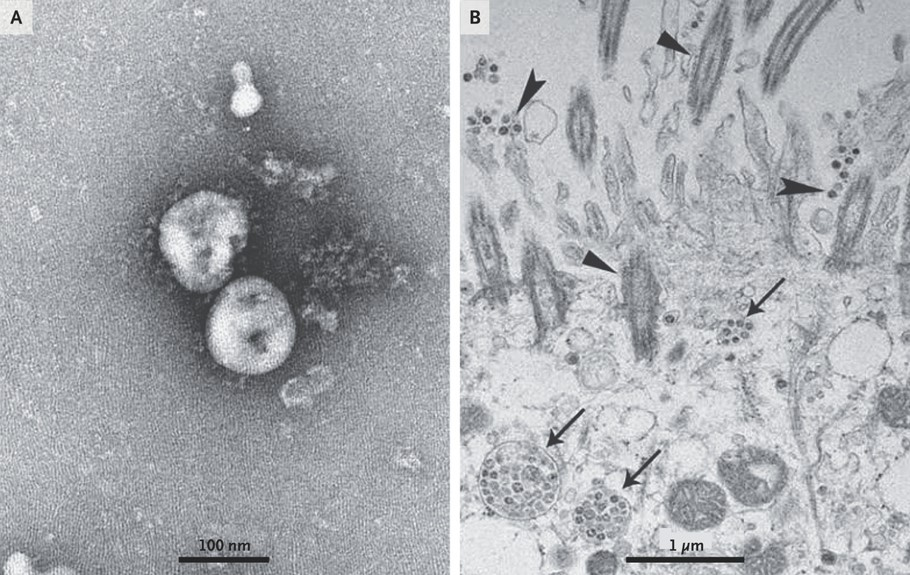
\includegraphics[width=\linewidth]{nCoV.jpg}
  \caption{Visualization of 2019-nCoV with Transmission Electron Microscopy  \cite{Zhu2020}.}
  \label{fig:2019-nCoV}
\end{figure}

\begin{thebibliography}{10}

\bibitem[Lee and Liu, 1980]{lee1980}
  Lee, KW and Liu, BYH,
  \textit{On the minimum efficiency and the most penetrating particle size for fibrous filters},
  Journal of the Air Pollution Control Association,
  \textbf{30}
  4
 (1980)


\bibitem[Zhu \textit{et al.}, 2020]{Zhu2020}
Zhu, Na and Zhang, Dingyu and Wang, Wenling and Li, Xingwang and Yang, Bo and Song, Jingdong and Zhao, Xiang and Huang, Baoying and Shi, Weifeng and Lu, Roujian and Niu, Peihua and Zhan, Faxian and Ma, Xuejun and Wang, Dayan and Xu, Wenbo and Wu, Guizhen and Gao, George F. and Tan, Wenjie,
\textit{A Novel Coronavirus from Patients with Pneumonia in China, 2019},
New England Journal of Medicine,
\textbf{382}
8 
(2020)
10.1056/NEJMoa2001017

\end{thebibliography}

\end{document}
